\documentclass[12px]{report}

%
%   Packages
%
\usepackage[a4paper,top=2cm,bottom=2cm,left=2cm,right=2cm]{geometry}
\usepackage{graphicx}
\usepackage{caption}
\usepackage{subcaption}
\usepackage[sorting=none]{biblatex}
\usepackage[acronym]{glossaries}
\usepackage[english]{babel}
\usepackage{csquotes}
\usepackage{setspace}
\usepackage{makecell}
\usepackage{float}
\usepackage{minted}

%
%   Line spacing
%
\setstretch{1.5}


%
%   Utilities and costants
%
\def\blankpage{
    \clearpage
    \thispagestyle{empty}
    \addtocounter{page}{-1}
    \null
    \clearpage
}

%
%   Acronyms
%
\newacronym{aria}{ARIA}{\textit{Air Pollutants Monitoring Using UAVs}}
\newacronym{cots}{COTS}{\textit{Commercial off-the-shelf}}
\newacronym{uavs}{UAVs}{\textit{Unmanned Aerial Vehicles}}
\newacronym{wsn}{WSN}{\textit{Wireless Sensor Network}}
\newacronym{epa}{EPA}{\textit{Environmnetal Protection Agengy}}
\newacronym{gso}{GSO}{\textit{Ground Station Operator}}
\newacronym{gcs}{GCS}{\textit{Ground Control Station}}
\newacronym{adc}{ADC}{\textit{Analog to Digital Converter}}
\newacronym{uart}{UART}{\textit{Universal Asynchronous Receiver-Transmitter}}
\makenoidxglossaries

%
%   References
%
\addbibresource{formats/references.bib}

%
%   Document
%
\begin{document}
    \begin{titlepage}
  \begin{center}
    \includegraphics[width=0.3\textwidth]{images/unipd.png}
    \hfill
    \includegraphics[width=0.3\textwidth]{images/dei.png}
  \end{center}
  \begin{center}
    \vspace{3cm}
    \large
    \MakeUppercase{
      \textbf{
        Dipartimento di ingegneria dell'informazione\\
        \vspace{0.5cm}
        Corso di laurea in Ingegneria Informatica\\
      }
    }
    \vspace{4cm}
    \MakeUppercase{
      \textbf{
        Acquisition and processing software for air pollution measurement on board drones of A.R.I.A. project\\
      }
    }
    \vspace{4cm}
    \begin{flushleft}
      \textbf{
        Thesis supervisor: Prof. Carlo Bettanini Fecia di Cossato\\
      }
    \end{flushleft}
    \vspace{1cm}
    \begin{flushright}
      \textbf{
        Candidate: Giacomo Favaron\\
      }
    \end{flushright}
    \vspace{2.5cm}
    \MakeUppercase{
      \textbf{
        Academic Year: 2020-2021\\
      }
    }
    \vspace{0.5cm}
    \textbf{
      Graduation Date: 11/15/2021
    }
  \end{center}
\end{titlepage}
    %\blankpage
    \begin{abstract}
In the recent years, awareness of the issue of Environmental Pollution has increased, and research shows that not enough has been done, until now, to reduce pollution. In this domain, the monitoring of air quality is fundamental to provide data which can be used to most effectively guide our efforts to reduce air pollution. At this time the monitoring of air quality is usually performed via stationary ground-mounted air pollution stations. However, research(??) has shown that air pollution can vary greatly at different heights, for this reason the \gls{aria} project is aiming to develop a system to measure vertical gradients of air pollutants using vertical swarms of drones. The \gls{aria} project solution is a low-cost monitoring system based on \gls{cots} sensors and on multiple cheap drone platforms. The system is equipped with $PM_2.5$ and $PM_10$ sensors to monitor the particulate concentration and several other gas sensors (such as $NO$, $NO_2$, $CO$, etc.) and the use of \gls{uavs} allows to build a 3D map of pollutants in a specific area. This could prove very useful around buildings in urban areas and possibile polluting plants in industrial areas. In this thesis are presented the system platform, the software implementation and a test flight.
\end{abstract}
    \clearpage
    \tableofcontents{}
    \clearpage
    \listoffigures
    \clearpage
    \printnoidxglossary[type=acronym, title={List of abbreviations}, style=index, nonumberlist]
    \printacronyms
    \clearpage
    \chapter{Introduction}
% TODO:
% - Trovare ref punti di domanda
Air pollution is caused by different typologies of gas pollutants that are present in the first meters (< 150 m) of the atmosphere and cause therefore damages to humans and environment. As air pollution is becoming the largest environmental health risk, the monitoring of air quality has drawn much attention in both laboratory studies and specific field tests and data collection campaigns. Government agencies and local administrations have, generally, provided and used monitoring stations on dedicated sites in cities and urban areas. Usually the studies have been conducted using fixed stations that are very reliable but produce only coarse-grained 2D monitoring, with several kilometers between two monitoring stations; or the stations monitor the same local area for long periods.
Other approaches show that applications using simple system of sensors have been developed to monitor the fine-grained air quality using densely deployed sensors [? ], [? ]. In any case, the fixed sensor station may achieve high precision, but have high cost and require maintenance and suffer especially for lack of mobility.
Furthermore, these approaches don't account for the vertical gradients of air pollution levels. As shown in research (?, ?) the concentrations of air pollutants can vary greatly at different heights and this is a sensitive factor in circumstances such as buildings in urban areas and possible polluting plants in industrial areas.
The usage of Unmanned Aerial Vehicles (UAVs) has been particularly rich in the latest years due to their flexibility, mobility and affordable cost. Current monitoring systems are not able to satisfy every need of modern cities and industrial areas and UAVs are valuable supporting elements in this scenario.
In terms of urban conditions, which is the main subject of the present study, UAVs can be used to measure environmental parameters such as illumination, wind speed, temperature, humidity, air quality [? ] and much more. In any case, for a complete analysis, both ground sensing and aerial sensing are necessary to provide 3D mapping and gas profiling. In our ARIA project, we equipped with the same set of sensors the devices that execute sensing on the ground, and the systems that execute aerial sensing on board the \gls{uavs}, which we are deploying in vertical swarms, to measure pollution levels at different heights.
The fixed ground sensing suite is able to collect data in a continuous way, but the air quality of the higher levels of air off the ground cannot be detected, so the contemporary use of drones is mandatory. Aerial sensing, on the contrary, is able to sense the air quality off the ground, but it cannot be executed for very long periods due to the high consumption of battery power and human time. By merging the potentialities of these two systems of sensing suites, a better set of data can be collected [? ]. A trade off on the possible sensors and UAVs has been performed and quadcopters are the preferred platform for monitoring because of their simplicity, low cost and hovering capabilities. On the contrary a possible bias of data is due to the the influence of air jets created by the rotor rotation or by the electromagnetic field generated by the antennas present on board. The problem of choosing the best location of the sensors is examined in [? ] based on the physical structure of the drones. Our approach is to use an extension on which we fix the sensors in order to suck the air away of the main air jets.
\section{Related works and state of the art}
\subsection{Air Pollution}
According to \cite{epc} "Air pollution can be defined as the presence of toxic chemicals or compounds (including those of biological origin) in the air, at levels that pose a health risk. In an even broader sense, air pollution means the presence of chemicals or compounds in the air which are usually not present and which lower the quality of the air or cause detrimental changes to the quality of life (such as the damaging of the ozone layer or causing global warming)".
Air pollution is extremely complex to evaluate and there are many polluting substances in the atmosphere. The \gls{epa} (of United States) takes these 6 (the "criteria air pollutants") in consideration in its studies:
\begin{table}[h!]
\caption{Criteria air pollutants and their health effects \cite{7946542}}
\centering
\begin{tabular}{ |c|c|c|c| }
    \hline
    \thead{Chemical symbol} & \thead{Substance} & \thead{Characteristics} & \thead{Effect} \\ [0.5ex]
    \hline
    \hline
    CO & Carobon Monoxide & Colorless, odorless gas & \makecell{Reducing oxygen delivery to the \\ body's orogans and tissues} \\
    \hline
    $NO_2$ & Nitrogen Dioxide & Highly reactive gas & \makecell{Risk of emphysema, asthma \\ and bronchitis diseases} \\
    \hline
    $O_3$ & Ozone & Pale blue gas & \makecell{Chest pain, coughing, \\ throat irritation} \\
    \hline
    $SO_2$ & Sulfur Dioxide & Colorless, irritating smell gas & \makecell{Risks of bronchoconstriction \\ and increase of asthma symptoms} \\
    \hline
    $PM_2.5$ and $PM_10$ & Particulate Matter & Inhalable particles & \makecell{Premature death and respiratory \\ symptoms} \\
    \hline
    Pb & Lead & Metal particles & \makecell{Accumulate in bones and \\ affecting the nervous system} \\ [1ex]
    \hline
\end{tabular}
\label{table:airpollutants}
\end{table}
\subsection{Air quality monitoring}
Air quality monitoring is an essential part in order to know what measures to put in place \cite{who-airquality} to protect our health and the environment, which are strongly connected.
In the Veneto region, Italy, the area of this study, the ARPAV\cite{arpav} has put in place a conventional monitoring network to track major air pollutants and enforce restrictory measures on polluting factors (such as transportation) if necessary. Figure \ref{fig:arpav-map} shows the map of ARPAV's current 2D monitoring network, which gives an example of the very low spacial resolution of conventional air quality monitoring systems.
\begin{figure}[h!]
    \centering
    \includegraphics[width=0.7\textwidth]{images/ARPAV stazioni rete 2019.jpg}
    \caption{ARPAV monitoring netowrk in the Veneto region, Italy\cite{arpav}}
    \label{fig:arpav-map}
\end{figure}
\subsection{Low-cost sensors}
The \gls{epa} also provides the Air Sensor Guidebook\cite{williams2014air} which gives extensive information on air quality and low-cost sensors. Due to their prohibitive cost and complexity, conventional air pollution monitoring systems have low spacial and temporal resolution. Low-cost sensors, instead, can be deployed more diffusely with high spacial and temporal resolution, while trading most of their accuracy. They are, in fact, heavily influenced by many factors, especially temperature, humidity, wind and presence of other gases in the air.  Due to their lightweight, only low-cost sensors can be mounted on drones: the aforementioned influence factors could introduce even more inaccuracy, especially wind generated from the rotors.
\cite{s151229859} among other things presents an evaluation of air quality sensors classifying their performances by the most important parameters.
\subsection{Drone systems}
Coordinating data collection and movements is quite hard, considering the low computational power of UAVs, the inaccuracy of GPS and the general wireless communication issues. Ref [5] is a survey on the communication issues releted to drone networks. The energy constraint is really impactful on long missions and poses a major limitation to the spreading of drone technology. Drones have excellent mobility and data gathering prowess, but cannot always rely on coming back to the base to deliver their information. Implementing reasonable communication protocols and algorithms is necessary to improve efficiency. 
\subsection{Drone monitoring and sensing}
Thanks to their mobility and flying movement, drone monitoring and sensing capabiliteis are very valuable. In urban settings \gls{uavs} can monitor noise, traffic, light, wind, temperature, humidity, air quality and many other parameters.
As shown earlire, conventional air quality monitoring systems have very low spatial and temporal resolution. \gls{uavs} based systems could measure specific areas with great convenience and felxibility and hybrid ground and air based solutions could routinely track the air pollution levels of parts of a city. \cite{7946542}, \cite{evangelatos2015airborne}, \cite{8675167}, \cite{8662050} propose different solutions for a \gls{wsn} using \gls{uavs}. \cite{8675167} in particular examines an application in smart cities, where a hybrid ground and air based system tracks an urban area.
\section{Dissertation structure}
This dissertation describes the \gls{aria} project solution for the monitoring of air pollution. It is divided into 6 chapters:
\begin{itemize}
    \item Chapter 1 describes the introduction, an overview on the topic of air pollution, the motivation to approach the problem, the motivation of the proposed solution, related works, the state of the art and the dissertation objective.
    \item Chapter 2 describes the system architecture, that is the \gls{uavs} that are being used, their design, specifications and functionality.
    \item Chapter 3 describes the sensor payload, the motivation of the adopted sensors and their use.
    \item Chapter 4 describes the software implementation for the data collection of the sensors and the communication of the \gls{uavs}.
    \item Chapter 5 shows the results of a test flight using the proposed solution.
    \item Chapter 6 presents what conclusions can be taken after all the developed work, and what improvements can be done in the future.
\end{itemize}
\section{Dissertation objective}
The objective of this dissertation is to describe the solution proposed by the \gls{aria} project for air pollution monitoring, in particular the software impelementation, to show preliminary results and discuss their revelance in future applications.
    \clearpage
    \chapter{ARIA project}
\section{Overview}
ARIA project was created by a group of students from the Department of Industrial Engineering, University of Padova, under the suggestion and guidance of personnel staff of the Center for Space Studies and Activities (CISAS) of the same University. The core motivation that brought together these students was the desire of researching new fields of application for drone technology.ARIA project’s scenario is investigation about drones usage within air quality monitoring. Environmental pollution is becoming every day more threatening for our health and we wanted to develop a tool to monitor it in 3D. the project is funded by the Department of Industrial Engineering of our University.
\section{Proposal presentation}

As for system which use only \gls{uavs}, however, a single UAV, is very limited in its performance due to its coverage, energy autonomy and small selection of sensors.  Swarms, instead, can provide full coverage of an area, while coordinating the best routes to visit each sensing node. Equipping different drones with different sensors is far easier and more flexible than having one doing everything on its own. The differentiating factor of the \gls{aria} project solution is the use of vertical swarms to monitor pollution at different heights, which is not a popular topic.
    \clearpage
    \chapter{ARIA: System architecture}
The selected system is a compromise between payload capacity, in-flight stability and
manoeuvrability and low-cost. The system is composed by:
\begin{itemize}
    \item Tarot 650 Sport drone, for the platform
    \item Hex Cube Black Flight Controller
    \item HERE2 GPS system
    \item Raspberry Pi3b+ for the controller devoted to sensor measurement
    \item A suite of sensors for air quality monitoring (in particular NO, NO2, CO and VOCs) based on Alphasesnse AFE board
    \item Nova SDS011 PM board to measure PM2.5 and PM10
    \item Taranis 9D+ Radio and an 8XR receiver
\end{itemize}
\begin{figure}[h!]
    \centering
    \includegraphics[width=1\textwidth]{images/system-architecture.png}
    \caption{\gls{aria} drone system components}
    \label{fig:aria-drone}
\end{figure}
The ARIA Project is going to use
simultaneously two drones and a fixed ground station, equipped with the same instrumentation in
order two build a 3D map of the investigated area. We are currently experimenting with the use of an Arduino controller on the second drone to compare the data collected by a different platform and allow the presence of additional sensor (such as temperature) thanks to Arduino's support of an higher number of input channels. This dissertation will focus on the Rapberry based system.
There has been just some laboratory testing on the effect of the blade disturbances on the measurement \cite{8453584}
but a comprehensive study on sensor location on such platforms has not been done yet; therefore
the ARIA project has designed a vertical boom were all the gas sensors are located. On the other
hand, in the area above the UAV, there is a relatively constant air flow which drops significantly after
a distance of approximately 40.0-50.0 cm for devices with characteristics similar to those used in the
proposed solution. The airflow behaviour is similar aside from the UAV in the area with a radius from
the center r $>$ 50.0 cm. To avoid the swirl area, it is recommended to place horizontal and vertical
probes of the appropriate length. The use of horizontal probes often makes it difficult to achieve the
conditions necessary for isokinetic sampling. In addition, it is necessary to use additional structures for their equalization. To overcome this problem, it was decided to use the vertical probe; the use of a
boom in a vertical position does not affect the flight capabilities of the UAV since the entire system has
a low center of mass, situated in the proximity of the battery.
Figure \ref{fig:aria-drone} contains an overview of the various system components; while Figure \ref{fig:system} shows one of the drones and some details of the system.
The UAV pilot or the UAV \gls{gso} can communicate with the UAV
wirelessly, using a radio controller (RC) transmitter or a computer, respectively.
Power is provided by a 6s Lipo battery able to give 10000mAh. Communication
between the flight controller and ground station is via 433MHz telemetry link connected to a laptop; a
2.4GHz communication link is also ensured via the Taranis 9D+ Radio and an 8XR receiver onboard the
UAV.
\clearpage
\begin{figure}[!ht]
    \centering
    \begin{subfigure}[b]{0.45\textwidth}
        \centering
        \includegraphics[width=\textwidth, angle=-90]{images/drone/IMG_20211105_103832.jpg}
        \caption{}
        \label{fig:wide}
    \end{subfigure}
    \hfill
    \begin{subfigure}[b]{0.45\textwidth}
        \centering
        \includegraphics[width=\textwidth, angle=-90]{images/drone/IMG_20211105_103729.jpg}
        \caption{}
        \label{fig:auto}
    \end{subfigure}

    \begin{subfigure}[b]{0.45\textwidth}
        \centering
        \includegraphics[width=\textwidth, angle=-90]{images/drone/IMG_20211105_103839.jpg}
        \caption{}
        \label{fig:rasp}
    \end{subfigure}
       \caption{The Rasperry Pi \gls{aria} drone}
       \label{fig:system}
\end{figure}

    \clearpage
    \chapter{Sensor Payload}
The sensor payload is composed by 3 subsystems:
\begin{enumerate}
    \item Raspberry Pi 3b+
    \item Analogue Front End (AFE) by Alphasense equipped with 3 gas sensors (NO, NO2 and CO) and a PID (VOCs) sensor
    \item Nova SDS011 particulate sensor board for PM2.5 and PM10
\end{enumerate}
A student bachelor thesis performed a FEM study on the sensors and the Pi3b+ support platforms. The
elements have been studied in order to present a high resistance to vibrations and to allow the sensors
and the boards to be housed in the most safest way. In addition, the study also sought to design very
light components: the boards were built with a 3D PLA printer in order to host in a compact and
reliable way all the instrumentation (see Figure \ref{pla}).
\begin{figure}[h!]
    \centering
    \begin{subfigure}[b]{0.45\textwidth}
        \centering
        \includegraphics[width=\textwidth]{images/drone/IMG_20211105_103941.jpg}
        \caption{}
        \label{fig:pla1}
    \end{subfigure}
    \hfill
    \begin{subfigure}[b]{0.45\textwidth}
        \centering
        \includegraphics[width=\textwidth, angle=-90]{images/drone/IMG_20211105_115556.jpg}
        \caption{}
        \label{fig:pla2}
    \end{subfigure}
       \caption{The 3D printed boards}
       \label{fig:pla}
\end{figure}
\clearpage
\section{Particulate sensors}
The particulate sensor is a Nova SDS011 PM sensor able to measure PM2.5 and PM10
concentrations with a resolution of $0.3\mu g/m^3$; range of measurement is: $0 - 1 mg/m^3$ and the frequency
of output is 1 Hz. The sensor is a \gls{cots} sensor used for house and environmental monitoring with
consumption around 1 W. Tests on the sensor were performed in the lab and outputs were calibrated.
The sensor is equipped with a 10 cm inlet pipe (see Figure 2) in order to facilitate the inflow of the air
in the sensor. Sensor is linked to the Raspberry via a USB interface board allowing fast connection and
is located on the drone main platform.
\begin{figure}[h!]
    \centering
    \includegraphics[width=0.7\textwidth]{images/drone/IMG_20211105_104126.jpg}
    \caption{The SDS011 particulate sensor and it's USB connected to the Raspberry Pi (partially covered by the pole structure)}
    \label{fig:sds011}
\end{figure}
\clearpage
\section{Gas sensors}
\begin{table}[H]
    \caption{\gls{aria}'s gas sensors}
    \centering
    \begin{tabular}{ |c|c|c|c|c| }
        \hline
        \thead{Substance} & \thead{Sensor} & \thead{Weight [g]} & \thead{Range [ppb]} & \thead{Data sheet} \\ [0.5ex]
        \hline
        \hline
        $CO$ & Alphasense CO-A4 & $< 6$ & 500 & \cite{co-a4} \\
        \hline
        $NO$ & Alphasense NO-A4 & $< 6$ & 20 & \cite{no-a4} \\
        \hline
        $NO_2$ & Alphasense NO-A43F & $< 6$ & 20 & \cite{no2-a43f} \\
        \hline
        $VOCs$ & Alphasense PID-AH2 & $< 8$ & \makecell{40 \\ (isobutylene)} & \cite{pid-ah2} \\
        \hline
    \end{tabular}
    \label{table:ariasensors}
\end{table}
They are connected to the Adafruit ADS1115 ADC and then to the raspberry. Due to 
The gas sensors have been positioned on a 50 cm boom in the center of the drone main platform
and above the drone itself (see Figure 2) in order to reduce disturbances due to variable flux moved
by the blades. Preliminary analysis show that the sensors are located in a non-altered flux allowing
for reliable measurements. Due to possible disturbances from electromagnetic sources present on the
drone (mainly telemetry antennas and electronics) a Faraday cage, not present in this study, but will be
built around the gas sensors and tested in future flights.
\begin{figure}[h!]
    \centering
    \begin{subfigure}[b]{0.45\textwidth}
        \centering
        \includegraphics[width=\textwidth]{images/drone/IMG_20211105_104008.jpg}
        \caption{}
        \label{fig:gas-sensors1}
    \end{subfigure}
    \hfill
    \begin{subfigure}[b]{0.45\textwidth}
        \centering
        \includegraphics[width=\textwidth]{images/drone/IMG_20211105_104040.jpg}
        \caption{}
        \label{fig:gas-sensors2}
    \end{subfigure}
       \caption{The Alphasense gas sensors on the AFE board on top of the pole and the ADS1115 ADC on the side. The NO sensor is present but not connected.}
       \label{fig:gas-sensors}
\end{figure}
\clearpage


%sincronia con altro sistema arduino
%righe csv coerenti e synch
% picchi co semaforo, parco
%pm coincide, differenza data da pipetta
    \clearpage
    \chapter{Flight Control}
There are two computers on board the \gls{aria} system:
\begin{itemize}
    \item Hex Cube Black flight controller, to control the UAV.
    \item Raspberry pi 3b+ as a companion computer, for additional communication with the \gls{gcs} and the sensor data acquisition.
\end{itemize}
\section{Hex Cube Black}
The Cube autopilot is a flexible autopilot intended primarily for manufacturers of commercial systems. It is based on the Pixhawk-project (opens new window) FMUv3 open hardware design \cite{ardupilot}. It is the core of the UAV, all the main components needed for the flight (rotors, battery, receiver) are connected to its board and it handles all the processing needed to control the UAV.
\begin{figure}[H]
    \centering
    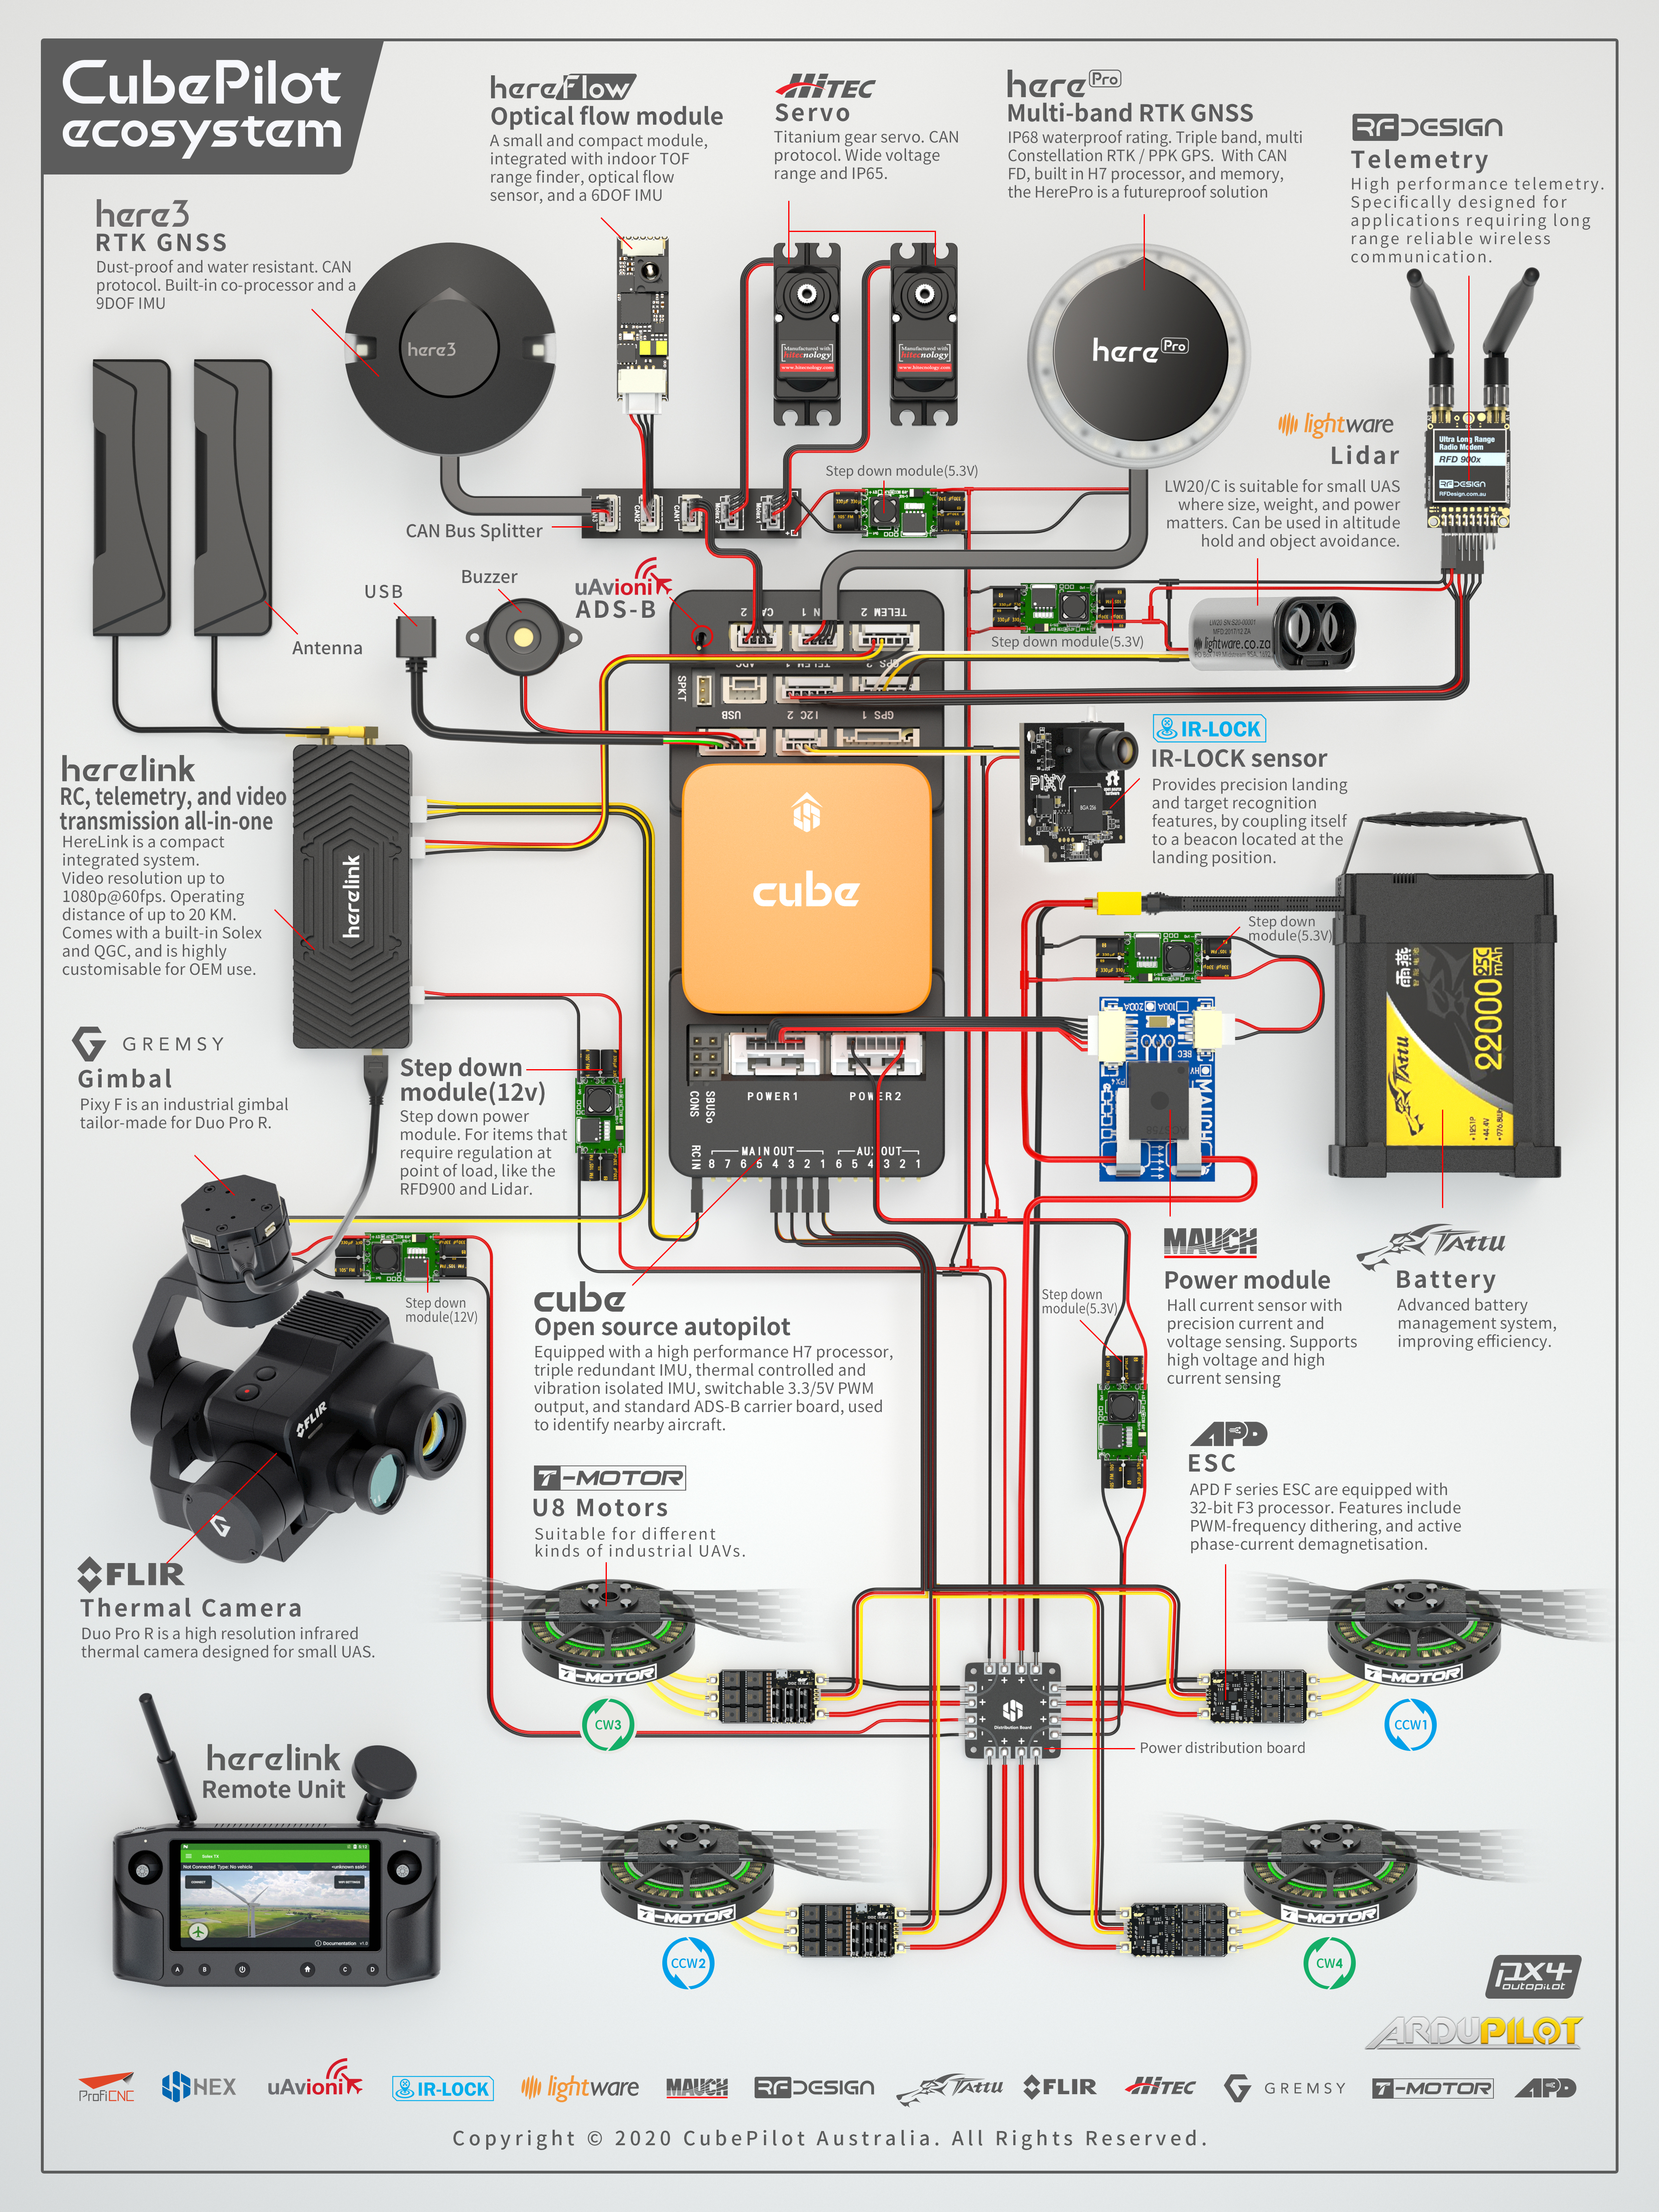
\includegraphics[width=0.4\textwidth]{images/cubepilot-ecosystem.jpg}
    \caption{The Cubepilot Ecosystem\cite{ardupilot}}
    \label{fig:cubepilot-ecosystem}
\end{figure}
The Hex Cube Black is an ArduPilot compatible autopilot.
\section{ArduCopter}
The firmware that the Pixhawk runs is the Arducopter, the copter specific version of ArduPilot, it is an open source firmware that supports the fully autonomous waypoint based flight and real time control, using MAVLink protocol to communicate with the Remote \gls{gcs}. The \gls{gcs} software used is Mission Planner.
\section{Mission Planner}
Mission Planner is a full-featured ground station application for the ArduPilot open source autopilot project \cite{ardupilot}.
It is used to configure the vehicle and plan the missions.
\begin{figure}[H]
    \centering
    \includegraphics[width=0.7\textwidth]{images/mission-planner.PNG}
    \caption{Screenshot of Mission Planner main screen, the gps is fixed in the laboratory location and the telemetry data is shown.}
    \label{fig:mission-planner}
\end{figure}

    \clearpage
    \chapter{Sensor Data Acquisition}
In the \gls{aria} project system the air pollution sensors are connected to the Raspberry pi companion computer, which reads the data and saves it along with the telemetry data received from the autopilot. My role when I joined the \gls{aria} project was writing the necessary code to achieve this reading and saving.
Figure \ref{fig:sensor-diagram} shows a diagram of the sensors architecture.
\begin{figure}[H]
    \centering
    \includegraphics[width=0.7\textwidth]{images/sensor-diagram.png}
    \caption{\gls{aria} sensors architecture}
    \label{fig:sensor-diagram}
\end{figure}
The task can be divided into 2 main parts:
\begin{enumerate}
    \item Reading and saving the data from the gas and particulate sensors.
    \item Connecting the Raspberry Pi to the pixhawk autopilot and receive the telemetry data through the MAVLink protocol.
\end{enumerate}
\section{Sensor data reading and saving}
\label{section:software}
Figure \ref{fig:sensor-diagram} also shows the connections between the various components of the system. The gas sensors are connected to the Raspberry Pi via the ADS115 \gls{adc} which is in turn connected to the i2c bus on the Raspberry. The SDS011 particulate sensor is instead connected via USB.
The code to read from these sensorse was written in Python3 (from now on referred to as Python for simplicity) and uses the official Adafruit Python ADS1x15 library and a custom Python based client for the SDS011 sensor.
The script (\texttt{aria.py}), after checking the connection with the components, continuously reads the data from the sensors. In the case of the gas sensors data received from the ADS1115, the raw data is also directly processed using specific formulas which were sent to us by Alphasense (Alphasense AAN 803-05, see Appendix \ref{chapter:formulas} for specifications). These formulas take in input the raw electrode readings (in mV, two per gas sensor) and output the measured gas concentration (in ppb), and include a series of parameters which depend on the specific serial number of the sensor and on the external temperature. Currently the Raspberry Pi based UAV only reads data from the NO2 and CO sensors since the ADS1115 only supports 4 channels and 2 channels are required for each sensor (for the two electrodes, "AE" and "WE" in the formulas). A larger module is going to be installed in the near future.
% The formulas we use for the processing of the NO2 and CO are:
% \begin{equation}
%     NO2 = ((WE_{NO2}-WE_{eNO2})-n_NO2*(AE_{NO2}-AE_{eNO2}))/sensNO_2
% \end{equation}
% \begin{equation}
%     CO = ((WE_{CO}-WE_{eCO})-n_CO*(AE_{CO}-AE_{eCO}))/sensCO
% \end{equation}
The data is then plotted in real time using the Python pyplot library and saved to a two different csv files, one with the raw sensor data, and the other for the processed sensor data. Every row contains also the date and time, the elapsed time since the acquisition script was started and the UNIX system time which is useful to check the synchronization with the data coming from the autopilot \ref{section:telem-data}. Figure \ref{fig:examples-script} shows examples of the terminal output, the live plot and the output csv files.
\begin{figure}[H]
    \centering
    \begin{subfigure}[b]{0.9\textwidth}
        \centering
        \includegraphics[width=0.8\textwidth]{images/cmd-and-plot.png}
        \caption{Screenshot of the terminal output and live plot while the script is running.}
        \label{fig:cmd-and-plot}
    \end{subfigure}

    \begin{subfigure}[b]{0.9\textwidth}
        \centering
        \includegraphics[width=\textwidth]{images/csv.PNG}
        \caption{Example of the output csv files, in particular the one with the telemetry data on the left, and the one with the sensors data on the right}
        \label{fig:csv}
    \end{subfigure}
       \caption{Examples of terminal output, live plot and output csv files from the main script aria.py}
       \label{fig:examples-script}
\end{figure}
\section{Telemetry data}
\label{section:telem-data}
To facilitate the processing of the data acquired during flight, we wanted to receive the telemetry data from the autopilot and temporally link it to the sensors data during flight. This would remove the need of a subsequent synchronization. To achieve this we connected the autopilot to the Raspberry Pi, which are both on board of the drone.
As shown in Figure \ref{fig:sensor-diagram} the Telem2 port on Hex Cube Black autopilot is connected to a serial port on the Raspberry Pi. Telem2 is the port on the Pixhawk for MAVLink communication.
\subsection{MAVLink protocol}
MAVLink is a very lightweight messaging protocol for communicating with drones and between onboard drone components. It is designed as a header-only message marshaling library.\cite{mavlink}.
\begin{figure}[H]
    \centering
    \includegraphics[width=0.7\textwidth]{images/mavlink-frame.png}
    \caption{MAVLink packet structure\cite{ardupilot}}
    \label{fig:mavlink-frame}
\end{figure}
Pixhawk and ArduPilot use MAVLink for communication. It is used between the Mission Planner \gls{gcs} software and the pixhawk, to control the UAV; and in the serial connection between the pixhawk and the Raspberry Pi companion computer, to send telemetry data.
MAVLink can transport messages and commands which are defined in a \textit{dialect}.
We used the common dialect defined in the official documentation\cite{mavlink-messages}, and the messages we needed were 'SYSTEM\_TIME' (ID \#2) and 'GLOBAL\_POSITION\_INT' (ID \#33). They, in fact, carry the UNIX time of the autopilot and telemetry data such as position, altitude and velocity. Figure \ref{fig:mavlink-messages} shows the exact content of the two messages.
\begin{figure}[H]
    \centering
    \includegraphics[width=0.8\textwidth]{images/mavlink-messages.png}
    \caption{MAVLink SYSTEM\_TIME and GLOBAL\_POSITION\_INT MAVLink messages\cite{mavlink-messages}}
    \label{fig:mavlink-messages}
\end{figure}
\subsection{Transmitting the data from the Hex Cube Black}
Firstly, through the Mission Planner, we configured the Telem2 port on the Hex Cube Black autopilot to use the MAVLink 2 protocol, as shown in Figure \ref{fig:telem2-protocol}. Serial2 is another name for the Telem2 port.
\begin{figure}[H]
    \centering
    \includegraphics[width=0.8\textwidth]{images/MP-Serial2_protocol.png}
    \caption{Configuration panel in Mission Planner, highlighted is the SERIAL2\_PROTOCOL parameter\cite{ardupilot}}
    \label{fig:telem2-protocol}
\end{figure}
And we set the SERIAL2\_BAUD parameter to 9, which sets the port baudrate to 9600.

The autopilot can send the data through the Telem2 port in 2 ways:
\begin{enumerate}
    \item After receiving a REQUEST\_DATA\_STREAM MAVLink message with the ID of the requested message.
    \item By setting appropriate parameters in the autopilot to have it continuously send groups of messages through the serial connection.
\end{enumerate}
We used the second method since we always needed the same messages to be sent (SYSTEM\_TIME and GLOBAL\_POSITION\_INT) and because this approach would remove the risk of lost packages. MAVLink, in fact doesn't guarantee the reception of messages.
At \cite{ardupilot-params} can be found the list of all the ardupilot parameters. The ones we needed were the 'SR2\_EXTRA3' and the 'SR2\_POSITION'. Setting these parameters to a non zero value (possible values 0-10Hz) has the autopilot send different groups of messages. Figure \ref{fig:ardupilot-groups} shows the messages in each group.
\begin{figure}[H]
    \centering
    \includegraphics[width=0.8\textwidth]{images/ardupilot-groups.png}
    \caption{SR2\_EXTRA3 and SR2\_POSITION data streams from ardupilot\cite{ardupilot-params}}
    \label{fig:ardupilot-groups}
\end{figure}
Through Mission Planner we set those parameters to 2Hz.
\subsection{Receiving the data on the Raspberry Pi}
The Telem2 port on the Hex Cube Black was connected to the \gls{uart} serial port on the Raspberry Pi 3b+ on pins GPIO 15 TxD (UART) and GPIO 16 RxD (UART). The serial connections was enabled in the Raspberry via \verb|raspy-config| and was available on \verb|/dev/ttyS0|.
On the Raspberry Pi the script responsible for reading from the serial port and decoding the MAVLink messages is \verb|mavlink_data.c|. It uses the official C library for MAVLink 2, c\_library\_v2, which contains the message definitions in XML format and helper functions to decode the messages.
The code reads form the \verb|/dev/ttyS0| serial port byte by byte; parses the message with the \verb|mavlink\_parse\_char| function; checks the ID of the parsed message and if the ID is either 2 (SYSTEM\_TIME) or 33 (GLOBAL\_POSITION\_INT) saves the information in the output csv file. The following code snippet contains the reading, parsing and decoding in the case of the SYSTEM\_TIME message.
\begin{minted}{c}
    while(1) {
        if(flag)
            break;
        int n = read (fd, &byte, 1);
        if(n == -1) {
            fprintf (stderr, "error %d on read: %s", errno, portname, strerror (errno));
            return 1;
        }
        if (mavlink_parse_char(chan, byte, &msg, &status)) {
            printf("Received message with ID %d, sequence: %d from component %d of system %d\n", msg.msgid, msg.seq, msg.compid, msg.sysid);
            switch(msg.msgid) {
                case MAVLINK_MSG_ID_SYSTEM_TIME: {
                    mavlink_msg_system_time_decode(&msg, &time_message);
                    mavlink_unix_time = time_message.time_unix_usec;
                    time_since_boot = time_message.time_boot_ms;
                    flag = true;
                }   
            }
        }
    }
\end{minted}
\section{Code overview}
The code is available at this Github repository\cite{repo}.
The structure of the main script (\verb|aria.py|) is the following:
\begin{verbatim}
    Open connection with the SDS011 sensor and the ADS1115 ADC
    Call mavlink_data.c to check connection with the autopilot
    Start an infinite loop:
        Call mavlink_data.c to get telemetry data
        Acquire data from particulate and gas sensors
        Process the data
        Write data to output csv files
        Real time plot of the data with pyplot
\end{verbatim}
At every iteration of the loop both telemetry and sensors data are collected, so the rows of the csv files are time synchronized.
    \clearpage
    \chapter{ARIA: Field Test}
A field test was performed in a trafficked area in Padova (Italy) in autumn 2021 (see Figure \ref{fig:3d-map}), mainly to test the sensors. The drones were carried by hand. the Figures below contain the data collected by the two drones, the mission times are synchronized and the Arduino drone also has the data for the NO sensor.


therefore data was collected at ground level except for the portion between xxx and xxx seconds when we set the drone on the bridge above the road at xxx m.

\begin{figure}[h!]
    \centering
    \begin{subfigure}[b]{0.45\textwidth}
        \centering
        \includegraphics[width=\textwidth]{images/flight-data/3d-map.jpg}
        \caption{}
        \label{fig:3d-map}
    \end{subfigure}
    \hfill
    \begin{subfigure}[b]{0.45\textwidth}
        \centering
        \includegraphics[width=\textwidth]{images/flight-data/raspberry/ALT_3D_R.jpg}
        \caption{}
        \label{fig:testflight-alt}
    \end{subfigure}
       \caption{3D map and 3D altitude plot}
       \label{fig:testflight-telemetry}
\end{figure}

\begin{figure}
    \centering
    \begin{subfigure}[b]{0.45\textwidth}
        \centering
        \includegraphics[width=\textwidth]{images/flight-data/raspberry/pms_R.jpg}
        \caption{Raspberry Pi drone PM sensor data}
        \label{fig:pms_R}
    \end{subfigure}
    \hfill
    \begin{subfigure}[b]{0.45\textwidth}
        \centering
        \includegraphics[width=\textwidth]{images/flight-data/raspberry/ariasensors_R.jpg}
        \caption{Raspberry Pi drone gas sensor data}
        \label{fig:ariasensors_R}
    \end{subfigure}

    \centering
    \begin{subfigure}[b]{0.45\textwidth}
        \centering
        \includegraphics[width=\textwidth]{images/flight-data/arduino/pms.jpg}
        \caption{Arduino drone PM sensor data}
        \label{fig:pms}
    \end{subfigure}
    \hfill
    \begin{subfigure}[b]{0.45\textwidth}
        \centering
        \includegraphics[width=\textwidth]{images/flight-data/arduino/ariasensors.jpg}
        \caption{Arduino drone gas sensor data}
        \label{fig:ariasensors}
    \end{subfigure}
    \hfill
       \caption{PM and gas sensors data from the Raspberry Pi drone (top two) and the Arduino drone (bottom two)}
       \label{fig:pms-and-sensors}
\end{figure}

\begin{figure}
    \centering
    \begin{subfigure}[b]{0.45\textwidth}
        \centering
        \includegraphics[width=\textwidth]{images/flight-data/raspberry/CO_3D_R.jpg}
        \caption{Raspberry Pi $CO$}
        \label{fig:CO_3D_R}
    \end{subfigure}
    \hfill
    \begin{subfigure}[b]{0.45\textwidth}
        \centering
        \includegraphics[width=\textwidth]{images/flight-data/raspberry/NO2_3D_R.jpg}
        \caption{Raspberry Pi $NO_2$}
        \label{fig:NO2_3D_R}
    \end{subfigure}

    \centering
    \begin{subfigure}[b]{0.45\textwidth}
        \centering
        \includegraphics[width=\textwidth]{images/flight-data/arduino/CO_3D.jpg}
        \caption{Arduino $CO$}
        \label{fig:CO_3D}
    \end{subfigure}
    \hfill
    \begin{subfigure}[b]{0.45\textwidth}
        \centering
        \includegraphics[width=\textwidth]{images/flight-data/arduino/NO2_3D.jpg}
        \caption{Arduino $NO_2$}
        \label{fig:NO2_3D}
    \end{subfigure}
    
    \begin{subfigure}[b]{0.45\textwidth}
        \centering
        \includegraphics[width=\textwidth]{images/flight-data/arduino/NO_3D.jpg}
        \caption{Arduino $NO$}
        \label{fig:NO_3D}
    \end{subfigure}
       \caption{3D plots of the gas sensors data, Raspberry Pi drone data is in blue (top two), Arduino drone data is in red (bottom three)}
       \label{fig:3Ds}
\end{figure}
    \clearpage
    \input{includes/conclusions.tex}
    \clearpage
    \printbibliography[
        heading=bibintoc,
        title={Bibliography}
    ]
\end{document}